\chapter{Theoretical Preliminaries}
\label{chap:preliminaries}

\section{Graph Theory Foundations}
\label{sec:graph_theory}

To computationally solve a routing problem across the European transit network, the physical infrastructure must be translated into a mathematical structure known as a graph. A graph $G = (V, E)$ is defined by a set of vertices $V$ (or nodes) and a set of edges $E$ that connect pairs of vertices.
In the context of transportation routing, a standard graph is inherently directed and weighted.

\medskip

\textbf{Directed edges.}
Transit connections are unilateral. An edge $e = (u, v)$ indicates a valid route from node $u$ to node $v$. The existence of $e = (u, v)$ does not imply the existence of a return edge $e' = (v, u)$ at the same time or cost.

\textbf{Weighted edges.}
Each edge carries a cost, typically represented by a weight function $w(u, v)$. In our context, this weight represents temporal costs, such as the travel duration of a flight or the waiting time of a layover.

\medskip

A path in this graph is a sequence of vertices where each adjacent pair is connected by a valid edge. The goal of a routing algorithm is to find a specific path that maximizes or minimizes a certain objective function (e.g., minimizing total weight or maximizing the number of unique vertices visited).

\begin{figure}[htbp]
  \centering
  \begin{minipage}[t]{0.46\textwidth}
    \centering
    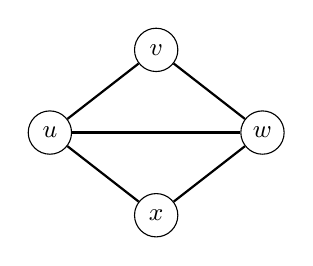
\begin{tikzpicture}[
        node/.style={circle, draw, inner sep=1.5pt, minimum size=5.5mm, font=\small},
        edge/.style={thick}
      ]
      \node[node] (u) at (0,0) {$u$};
      \node[node] (v) at (1.35,1.05) {$v$};
      \node[node] (w) at (2.7,0) {$w$};
      \node[node] (x) at (1.35,-1.05) {$x$};
      \draw[edge] (u) -- (v);
      \draw[edge] (v) -- (w);
      \draw[edge] (w) -- (x);
      \draw[edge] (x) -- (u);
      \draw[edge] (u) -- (w);
    \end{tikzpicture}
    \par\medskip
    {\small\textbf{(a)}~$G=(V,E)$ with $V=\{u,v,w,x,\ldots\}$ and $E=\{(u,v),(v,w),\ldots\}$.}
  \end{minipage}\hfill
  \begin{minipage}[t]{0.50\textwidth}
    \centering
    \begin{tikzpicture}[
        node/.style={circle, draw, inner sep=1.5pt, minimum size=5.5mm, font=\small},
        edge/.style={-{Stealth[length=2mm]}, thick},
        lbl/.style={font=\scriptsize, fill=white, inner sep=0.5pt}
      ]
      \node[node] (u) at (0,0) {$u$};
      \node[node] (v) at (2.0,0) {$v$};
      \node[node] (w) at (4.0,0) {$w$};
      \draw[edge] (u) -- node[lbl, above] {$95$} (v);
      \draw[edge] (v) -- node[lbl, above] {$40$} (w);
      \node[font=\scriptsize, align=center] at (2.0,-0.85) {$e=(u,v),\; e=(v,w)$};
      \node[font=\scriptsize] at (2.0,-1.35) {path: $u \to v \to w$};
    \end{tikzpicture}
    \par\medskip
    {\small\textbf{(b)}~$w(u,v)=95$, $w(v,w)=40$ (minutes); a routing algorithm searches for a path in $G$.}
  \end{minipage}
  \caption{Panel~(a) shows the abstract structure $G=(V,E)$; panel~(b) shows directed edges $e=(u,v)$ whose labels denote travel time in minutes, i.e.\ $w(u,v)=95$ and $w(v,w)=40$.}
  \label{fig:graph_foundations}
\end{figure}

\subsection{Time-Dependent vs.\ Time-Expanded Networks}
\label{subsec:time_expanded}

A traditional static graph is insufficient for modeling public transit because connections do not exist continuously; they are strictly bound to specific departure and arrival schedules. To model this dimension of time, routing problems typically rely on one of two paradigms:

\medskip

\textbf{Time-Dependent Networks.}
The physical topology of the graph remains static (e.g., one vertex per station), but the weight of an edge $w(u, v, t)$ is a function of the departure time $t$. This keeps the network compact, but complicates the routing algorithms, as the cost of traversal fluctuates dynamically.

\textbf{Time-Expanded Networks.}
Time is explicitly discretized and baked directly into the topology of the graph. A single physical station is duplicated into multiple vertices, each representing that station at a specific point in time (e.g., Station A at 10:00, Station A at 10:15). This dramatically increases the number of nodes and edges, but allows the use of standard, static routing algorithms, since every edge now possesses a fixed, immutable weight.

\medskip

Because our problem operates within a strict 24-hour window using discrete, fixed transit schedules, modeling time efficiently is the central architectural challenge. To systematically evaluate the optimal data structure for this Guinness World Record routing problem, this thesis intentionally implements and compares both paradigms: a memory-efficient time-dependent multi-graph (detailed in Chapter 4) and a structurally unrolled time-expanded network (detailed in Chapter 5). Similar comparisons have been made in the literature, see \cite{pyrga2007efficient}.

\subsection{Activity-on-Edge (AoE) vs.\ Activity-on-Node (AoN)}
\label{subsec:aoe_aon}

Beyond the choice of how to handle chronological time, transportation graphs must also dictate where the transit data physically resides within the topology. This relies on two distinct structural paradigms:

\medskip

\textbf{Activity-on-Edge (AoE).}
The traditional approach where vertices represent physical locations, and edges represent the actual transport activities (e.g., a train moving between two cities) or waiting periods. The temporal data is stored as attributes on the edges.

\textbf{Activity-on-Node (AoN).}
An inverted approach where the vertices themselves represent the specific transport activities (e.g., a flight with a fixed departure and arrival time), and the directed edges represent the valid layovers or transfer opportunities connecting them.

\medskip

Understanding the distinction between AoE and AoN is critical, as the choice of paradigm radically alters the branching factor, memory footprint, and traversability of the search space. A core objective of this research is to contrast these two frameworks directly. Chapter 4 evaluates a Time-Dependent AoE structure, while Chapter 5 introduces a structural pivot to a Time-Expanded AoN framework, allowing for a comparative analysis of their computational viability on a continental scale.

\section{Search and Optimization Algorithms}
\label{sec:search_algorithms}

When graph networks become too large for brute-force enumeration, exact and heuristic optimization algorithms are required to traverse the search space efficiently.

\subsection{Dynamic Programming and Label Setting}
\label{subsec:dp_label_setting}

Dynamic Programming is a mathematical optimization method that solves complex problems by breaking them down into simpler, overlapping subproblems. In the context of graph routing, DP is often implemented via Label Setting algorithms. As the algorithm traverses the graph, it assigns ``labels'' to each node, where a label represents the accumulated cost or state of a specific path reaching that node.

In multi-objective optimization problems, where multiple conflicting criteria must be optimized simultaneously (e.g., minimizing time while maximizing profit), a single optimal path cannot always be determined dynamically. Instead, the algorithm must maintain a Pareto Frontier at each node. The frontier is a set containing all non-dominated labels. A label $L_1$ mathematically ``dominates'' $L_2$ if it is equal or superior in all evaluated objectives, and strictly superior in at least one. Dominated labels are permanently discarded, while the non-dominated set is kept to spawn future branches.

\subsection{Depth-First Search (DFS) and Branch-and-Bound}
\label{subsec:dfs_bnb}

DFS is a fundamental graph traversal algorithm that explores as far down a single branch of a tree as possible before backtracking. Because DFS only requires storing the nodes along the current active path, its memory complexity grows linearly with the depth of the search tree rather than exponentially with its breadth, making it highly memory-efficient.

To optimize DFS for finding absolute maximums or minimums, it is often paired with Branch-and-Bound, a paradigm for discrete and combinatorial optimization.

\medskip

\textbf{Branching.}
The algorithm systematically divides the search space by exploring subsequent child nodes.

\textbf{Bounding.}
At each node, a bounding function calculates an optimistic mathematical estimate (an upper or lower bound) of the best possible solution that could be found by continuing down that branch.

\medskip

If the calculated bound of a branch is worse than the best solution already found elsewhere in the search (the incumbent solution), the algorithm instantly abandons the branch. This technique, known as pruning, eliminates vast sections of the search space without requiring explicit evaluation.

\section{Distributed Computing}
\label{sec:distributed_computing}

When a computational problem's scale exceeds the memory or processing capacity of a single machine, distributed computing methodologies are employed to divide the task across an HPC cluster. An HPC cluster is a network of independent computers (nodes) that function as a single system. Access to these resources is governed by a workload manager or job scheduler, such as SLURM (Simple Linux Utility for Resource Management). The scheduler allocates specific hardware constraints, such as CPU cores and maximum RAM, and queues tasks to ensure that execution does not exceed physical memory limits, which would otherwise trigger immediate task termination.

\medskip

To efficiently search massive combinatorial state spaces, algorithms frequently leverage data-level parallelism. In this paradigm, the exact same algorithm is executed concurrently across non-overlapping subsets of the initial data. In HPC environments, this is seamlessly orchestrated using job arrays. A job array takes a single execution script and duplicates it into dozens or hundreds of independent tasks, assigning each a unique environmental index. The algorithm uses this index to deterministically identify and process its specific slice of the search space, achieving massive throughput without the overhead of constant inter-node network communication.

\medskip

Within those individual tasks, intra-node multiprocessing is often utilized to fully saturate the assigned CPU cores. However, launching multiple concurrent processes can lead to severe memory duplication, which is fatal for memory-intensive graph traversals. To mitigate this, concurrent architectures employ IPC and shared memory. By utilizing thread-safe locks and shared variables, multiple worker processes can safely read global data structures and update shared states, such as a global incumbent bound, without triggering race conditions or redundant memory allocation.

\section{Data Acquisition Concepts}
\label{sec:data_acquisition_concepts}
To populate large-scale routing networks, real-world scheduling data must be extracted programmatically from remote servers. The standard mechanism for this is a REST API (Representational State Transfer Application Programming Interface). APIs provide structured endpoints where a client can send HTTP requests to retrieve specific, filtered datasets. In modern web architectures, this data is almost universally exchanged in JSON (JavaScript Object Notation), a lightweight, key-value serialization format. JSON allows nested, hierarchical data to be seamlessly transmitted over networks and deserialized directly into programmatic data structures, such as dictionaries and arrays, for immediate computational use.

\medskip

However, when public APIs are unavailable or heavily restricted, data must be gathered via web scraping. Web scraping involves automating HTTP requests to target servers and parsing the resulting HTML, a markup language designed for human-readable browsers rather than machine consumption. This requires algorithmic extraction of target variables from unstructured or semi-structured Document Object Model (DOM) trees. Both API querying and web scraping are strictly governed by server-side rate limits (throttling). Consequently, data acquisition pipelines must implement pagination logic, exponential backoff strategies, and fault-tolerant parsing to ensure reliable, large-scale dataset generation without triggering server bans or connection timeouts.